% $Id: circuit.tex 5861 2018-01-23 22:23:58Z mskala $

%
% MSK 010 circuit explanation
% Copyright (C) 2017, 2018  Matthew Skala
%
% This program is free software: you can redistribute it and/or modify
% it under the terms of the GNU General Public License as published by
% the Free Software Foundation, version 3.
%
% This program is distributed in the hope that it will be useful,
% but WITHOUT ANY WARRANTY; without even the implied warranty of
% MERCHANTABILITY or FITNESS FOR A PARTICULAR PURPOSE.  See the
% GNU General Public License for more details.
%
% You should have received a copy of the GNU General Public License
% along with this program.  If not, see <http://www.gnu.org/licenses/>.
%
% Matthew Skala
% https://northcoastsynthesis.com/
% mskala@northcoastsynthesis.com
%

\chapter{Circuit explanation}

The MSK~010 contains eight basically identical oscillators, differing only
in the resistor and capacitor values that determine their frequencies.  The
complete circuit for one of them is shown in Figure~\ref{fig:oscillator},
but to better understand the circuit, let's look at a simplified version
first.  Some of the component values have been changed (or filled in, where
they're unspecified on the main schematic) for a more understandable
presentation.

{\centering\input{wienbridge.tex}\par}

\begin{figure*}
\texdependspdfworkaround
\centering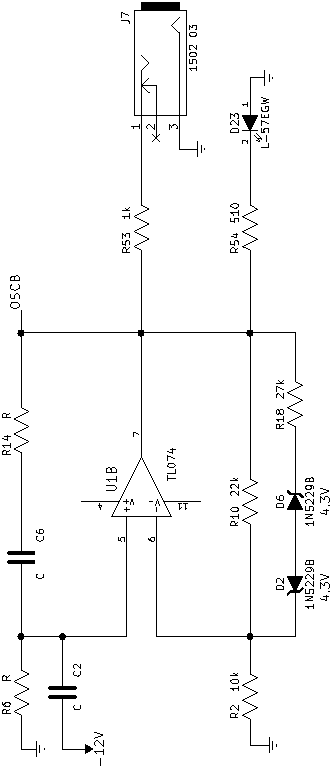
\includegraphics[height=\linewidth,angle=-90]{oscillator}\par
\caption{One oscillator.}\label{fig:oscillator}
\end{figure*}

This is the core of a ``Wien bridge oscillator,'' named for an
impedance-measuring circuit invented by Max Wien in 1891, which its feedback
network superficially resembles.  We can actually break it down even
further, into a noninverting amplifier:

{\centering\input{gain3.tex}\par}

and a voltage divider:

{\centering\input{vdiv.tex}\par}

Think about the voltage divider first.  At very low frequencies, capacitors
look like open circuits, with high impedance, infinite at zero frequency
(DC).  So for DC, the divider has infinite impedance on the top
(1M$\Omega$ in series with infinity) and 1M$\Omega$ impedance on the bottom
(1M$\Omega$ in parallel with infinity).  That gives zero output; no signal
from the input gets through.

At very high frequencies, capacitors have low impedance, going to a limit of
zero at infinite frequency.  So if we imagine feeding an infinite-frequency
signal into the voltage divider, it has 1M$\Omega$ impedance on the top
(1M$\Omega$ in series with zero) and zero impedance on the bottom
(1M$\Omega$ in parallel with zero).  Again, no signal gets through.

For frequencies that are neither zero nor infinite, the capacitors have
impedances that are also neither zero nor infinite, and then the voltage
divider lets through some amount of signal.  So now we have a rough
description of the behaviour of this circuit:  for high and low frequencies,
it blocks the signal, and for frequencies in between, it lets some signal
through.  It's a two-pole passive band-pass filter.

It is reasonably simple to show using calculus, though I will omit the
details here, there there must be some specific frequency in between zero
and infinity at which the output is maximized; and that frequency happens to
be the one where the capacitive reactance of the two capacitors is equal to
the resistance of the two resistors.  This is the centre frequency of the
band-pass filter.  Where $R$ is the value of each resistor and $C$ the value
of each capacitor, the centre frequency $f$ is given by
\begin{equation*}
  f = \frac{1}{2\pi RC} \, .
\end{equation*}

With the example values of 1M$\Omega$ and 0.1$\mu$F, this works out to
1.59Hz.

Now, how much signal actually does get through at the centre frequency?  At
1.59Hz, a 0.1$\mu$F capacitor has a capacitive reactance of 1M$\Omega$.  But
capacitive reactance is not the same as resistance; the two are actually at
right angles to each other on the complex plane.  Without going into a lot
of detail on that, we can get an intuitive understanding by saying that at
the centre frequency, the top of the voltage divider contains two 1M$\Omega$
impedances at right angles to each other, in series.  Series impedances add
as vectors, and adding two equal-length vectors at right angles to each
other gives a new one $\sqrt{2}=1.414\ldots$ the length of the inputs. 
(Pythagorean Theorem, 45-45-90 triangle.) So the top of the voltage divider
is an impedance with magnitude 1.414M$\Omega$.

On the bottom, we have two 1M$\Omega$ impedances at right angles to each
other in the complex plane, connected in parallel.  For parallel components,
the admittances (reciprocals of impedance) add as vectors.  So each of these
components has an admittance of 1$\mu$S (microsiemens, the inverse of
megaohms), and those add as right-angled vectors for an overall admittance
of 1.414$\mu$S for the pair of them, equivalent to an impedance with
magnitude 0.707M$\Omega$.

Just looking at the magnitudes of the top and bottom impedances in the
voltage divider, it looks like a 2:1 ratio, 1.414M$\Omega$ on top and
0.707M$\Omega$ on the bottom.  Then we can imagine that $1/3$ of the voltage
on the input might appear at the output.  This intuitive argument isn't
mathematically correct because it neglects the phases of the signals.  To
get a really correct result, we should calculate with complex numbers all
the way through, but if we do that, it turns out the intuitive estimate was
right after all: at the centre frequency, the voltage on the output really
is $1/3$ (as a pure real number, no phase shift) times the input voltage.

Now let's return to the amplifier.

{\centering\input{gain3.tex}\par}

This is a standard noninverting amplifier circuit built with an op amp.  The
input voltage is applied to the positive input of the op amp, and the op amp
will drive its output to whatever voltage is needed to make the negative
input match the positive input.  The negative input happens to be driven by
a voltage divider to $1/3$ of the output voltage; so the output voltage has
to be three times the input voltage, as long as the op amp is able to
sustain that.

The oscillator circuit combines this amplifier, with voltage gain 3, with
the resistor-capacitor band-pass voltage divider, which has voltage gain
$1/3$ at the centre frequency, and less at all other frequencies.  If there
happens to somehow already be a sine wave at the centre frequency on the op
amp output, then the band-pass voltage divider cuts its voltage by a factor
of three, and the amplifier boosts it back up to the original voltage.  So
the overall circuit can sustain oscillation at that frequency.  And
\emph{only} at that one frequency---because signals at any other frequency
will be attenuated more in the band-pass filter, then amplified with gain
only 3 in the amplifier, and so they come back at a reduced voltage each
time through the loop and die out completely after a few cycles.

But there are still a few problems.  How does the oscillation get started? 
If there is no signal at all, this circuit seems like it won't create one. 
How can we predict the amplitude of the signal?  And what about non-ideal
components?

If we are using real-life components, a 1M$\Omega$ resistor might be
specified as 1\%\ tolerance, and its actual value could be anywhere from
0.99M$\Omega$ to 1.01M$\Omega$.  If we are unlucky enough to get the
resistor (and, worse, the capacitor) on the top of the voltage divider a
little larger than its target, and also the components on the bottom a
little smaller, than the output of the voltage divider could be somewhat
less than $1/3$ the input voltage even at the frequency where the output
voltage is maximized.  And then if the amplifier really has gain of exactly
3 or less (less is quite possible because of tolerances in its own
resistors), the signal will come back a little weaker every time it goes
around the loop, and eventually die out.

So, we might make the gain of the amplifier a little more than 3 to
compensate for any extra losses that might exist in the rest of the circuit. 
With a 22k$\Omega$ feedback resistor matched against the 10k$\Omega$ to
ground, the gain becomes 3.2.

{\centering\input{gain32.tex}\par}

Now as long as the output of the voltage divider is more than about $0.31$
times the voltage divider's input, the amplifier will boost it above its
original level.  Any oscillation at the centre frequency will grow bigger
and bigger, without any obvious limit.

The op amp cannot produce an unlimited output voltage, so
something has to give.  What happens is that once the amplifier drives its
output to the maximum voltage it can handle (which would be about $\pm$9V
with the components and power supply used in the MSK~010), it stops acting
as a linear amplifier and starts producing distortion.  On an oscilloscope,
it looks like the tops and bottoms of the sine waves are getting clipped
off, leaving a roughly trapezoidal waveform.  In spectral terms, what is
happening is that some of the power is being diverted from the sine wave
into harmonic frequencies.  The harmonics will not make it through the
band-pass filter in any significant amounts, so they will not be re-amplified
as parasitic oscillations, but they get re-created on each pass from the
leftover power that cannot go into raising the voltage any further.

So, what can we do about this?  If the gain is too low, the oscillations
will die.  If the gain is too high, the op amp will be driven into clipping
and create a lot of distortion (as well as simply an output voltage higher
than we want).  And controlling the gain extremely precisely with
high-precision components and trimmers or similar, is expensive.  The
solution is to automatically reduce the gain a little as the voltage
increases.

{\centering\input{zeners.tex}\par}

At low output amplitudes, the output voltage stays near zero, and there is
never enough voltage across the back-to-back Zener diodes for them to
conduct.  That entire branch of the circuit has no effect, and the gain is
3.2.

At higher voltages, and in particular, once the output voltage goes past
8.6V peak to peak, the diodes will start to conduct.  Then current can flow
through them and R18 in addition to R10, reducing the effective resistance
in the feedback loop and therefore the gain.  At the extreme, for very high
output voltages the voltage drop across the diodes (maximum about 4.9V total,
for one reverse biased as 4.3V and the other forward biased at 0.6V) will be
negligible, and the feedback resistance will approach that of the parallel
combination of R10 and R18, namely about 12.1k$\Omega$.  That would give a
gain of 2.2 through the amplifier.

The output voltage never really goes that high, though.  What really happens
is that with very small signals, the gain is 3.2, causing the amplitude to
increase.  Once it gets to about 10V peak to peak, the increasing current
through the diodes cuts in R18 enough to reduce the gain to 3.0, and the
signal stabilizes at that amplitude.  If component imperfections, or changes
in value caused by temperature and aging, cause it to require a little more
or less gain, then the amplitude will increase or decrease a little until
the gain hits the right level for the oscillation to just sustain itself. 
Much the same thing happens in response to imperfections in the amplifier
circuit itself.

There is a price to be paid for this automatic adjustment:  the gain
is changing throughout the oscillation cycle (3.2 near zero crossings, 3.0
or slightly less at the peaks) and that means the amplifier is no longer
operating linearly.  Nonlinear amplifiers couple some of their output power
into harmonics.  As a result, there will be a bit of distortion in the
output.  In the MSK~010, especially given the intended application as a
modulation source, this distortion is small enough not to worry about.  But
if we wanted a \emph{really} pure sine wave, we would need an even cleverer
way of controlling the gain, with corrections applied throughout the cycle
over a longer period.

There is a tradition of using incandescent light bulbs for gain control in
Wien bridge audio oscillators, to the point that some people incorrectly
think the use of such is what makes it a Wien bridge oscillator.  The light
bulb would go in place of R2.  As output amplitude increases, the filament
heats up, which causes its resistance to increase, and therefore the gain
decreases.  It maintains a stable output level in the same way that the
MSK~010's Zeners do.  The time taken for the light bulb to heat up and cool
down is much longer than an oscillator cycle, so the gain is not changing
much during the cycle, and the distortion is very low.  Hewlett-Packard's
first product was a sine oscillator with this type of gain control.

Unfortunately, it's hard to get the right kind of incandescent light bulbs
anymore, they aren't compatible with modern electronic manufacturing
processes, and they wouldn't work in an LFO like the MSK~010 anyway because
the thermal time constant of the light bulb (a fraction of a second) needs
to be much longer than the oscillator cycle time (up to a minute in our
case).  But it remains a good trick to know about for the cases where it's
applicable.

Looking at Figure~\ref{fig:oscillator}, a few more refinements are apparent. 
For one thing, the capacitor in the band-pass filter is connected to the
negative power supply instead of to ground.  That is to help with startup;
without it, the oscillator would just be amplifying its own thermal noise
until that got to be enough to sustain oscillation, and that kind of
start-up takes longer than is desirable.  It's observable in practice with
the MSK~010 circuit on a breadboard, or with an ``oscillating filter'' type
of LFO such as an Intellijel Dr.\ Octature II: at initial power-up in LFO
mode, there's a delay, minutes long at the slowest setting, before the
lights light up.

Connecting the capacitor to -12V instead of ground means that at power-up
time, the oscillator will be much closer to its stable oscillating state. 
The capacitor is normally fully discharged at power-up.  Applying power
pulls the op amp negative input almost to the negative power rail, forcing
the output high and the amplitude-limiting Zener diodes to conduct at their
maximum.  Within a fraction of a cycle time, they have it on track at the
normal amplitude level.

One consequence of this design is that the -12V power supply needs to be
clean, because noise there can be coupled into the oscillator output---but
clean negative power is a general requirement of op amp circuits anyway, and
so is something we can hope for in a synth environment.  Another consequence
is that there will be a static DC charge of 12V on the capacitor.  That
means it's important to use a plastic film capacitor here and not a
ferroelectric ceramic type, which would suffer capacitance
degradation given a DC voltage like that.  But the need for close tolerance
on this timing capacitor pretty much already meant that we had to specify it
as plastic film anyway.

Also visible in the full schematic are the current-limiting resistor R53,
which prevents damage to other modules and disruption of the MSK~010's cycle
should the output get shorted out or patched into another output; and the
bi-colour LED D23 with its own current-limiting resistor R54.
